\documentclass[a4paper]{article}

\usepackage[font=small]{caption}
\usepackage{graphicx}
\usepackage[parfill]{parskip}

\begin{document}

2b) Starting from 1000 times of concatenation operations, StringBuilder approaches is bettern than the other.

\begin{table}[htbp]
\begin{tabular}{|l|l|l|}
\hline
\# of concatenation operations & Approach 1 (String) & Approach 2 (StringBuilder) \\ \hline
10                             & 0 ms                & 0 ms                       \\ \hline
100                            & 0 ms                & 0 ms                       \\ \hline
1000                           & 2 ms                & 0 ms                       \\ \hline
10000                          & 49 ms               & 1 ms                       \\ \hline
100000                         & 2042 ms             & 2 ms                       \\ \hline
\end{tabular} 
\captionsetup{justification=centering}
\caption*{Result for CompareLargeStringConcatenation}
\end{table}

3a) Result for CompareManySmallStringsConcatenation

\begin{table}[htbp]
\centering
\tiny
\setlength\tabcolsep{2pt}
\begin{tabular}{|c|cc|cc|cc|cc|cc|}
\hline
\multicolumn{1}{|l|}{\# of Strings / Operations} & \multicolumn{2}{c|}{0}        & \multicolumn{2}{c|}{1}         & \multicolumn{2}{c|}{2}          & \multicolumn{2}{c|}{3}          & \multicolumn{2}{c|}{4}          \\ \hline
Type of Approach                                               & \multicolumn{1}{c|}{A1} & A2  & \multicolumn{1}{c|}{A1}  & A2  & \multicolumn{1}{c|}{A1}   & A2  & \multicolumn{1}{c|}{A1}   & A2  & \multicolumn{1}{c|}{A1}   & A2  \\ \hline
1000                                                           & \multicolumn{1}{c|}{0 ms}  & 0 ms  & \multicolumn{1}{c|}{1 ms}   & 0 ms  & \multicolumn{1}{c|}{1 ms}    & 1 ms  & \multicolumn{1}{c|}{0 ms}    & 1 ms  & \multicolumn{1}{c|}{0 ms}    & 1 ms  \\ \hline
10000                                                          & \multicolumn{1}{c|}{0 ms}  & 1 ms  & \multicolumn{1}{c|}{0 ms}   & 1 ms  & \multicolumn{1}{c|}{1 ms}    & 1 ms  & \multicolumn{1}{c|}{2 ms}    & 1 ms  & \multicolumn{1}{c|}{3 ms}    & 0 ms  \\ \hline
100000                                                         & \multicolumn{1}{c|}{0 ms}  & 2 ms  & \multicolumn{1}{c|}{4 ms}   & 1 ms  & \multicolumn{1}{c|}{3 ms}    & 1 ms  & \multicolumn{1}{c|}{2 ms}    & 2 ms  & \multicolumn{1}{c|}{6 ms}    & 1 ms  \\ \hline
1000000                                                        & \multicolumn{1}{c|}{0 ms}  & 3 ms  & \multicolumn{1}{c|}{8 ms}   & 8 ms  & \multicolumn{1}{c|}{24 ms}   & 5 ms  & \multicolumn{1}{c|}{20 ms}   & 5 ms  & \multicolumn{1}{c|}{47 ms}   & 12 ms \\ \hline
10000000                                                       & \multicolumn{1}{c|}{5 ms}  & 29 ms & \multicolumn{1}{c|}{29 ms}  & 55 ms & \multicolumn{1}{c|}{110 ms}  & 41 ms & \multicolumn{1}{c|}{222 ms}  & 52 ms & \multicolumn{1}{c|}{295 ms}  & 66 ms \\ \hline
100000000                                                      & \multicolumn{1}{c|}{48 ms} & 247 ms & \multicolumn{1}{c|}{264 ms} & 315 ms & \multicolumn{1}{c|}{1076 ms} & 387 ms & \multicolumn{1}{c|}{1985 ms} & 519 ms & \multicolumn{1}{c|}{2939ms} & 659 ms \\ \hline
\end{tabular}
\captionsetup{justification=centering}
\caption*{(A1: Approach 1 (String). A2: Approach 2 (StringBuilder))}
\end{table}


3b) Approach 1 is the best when there is no concatenation operations at all on the strings. Starting from 100000 Strings, the difference between the approaches start to show.

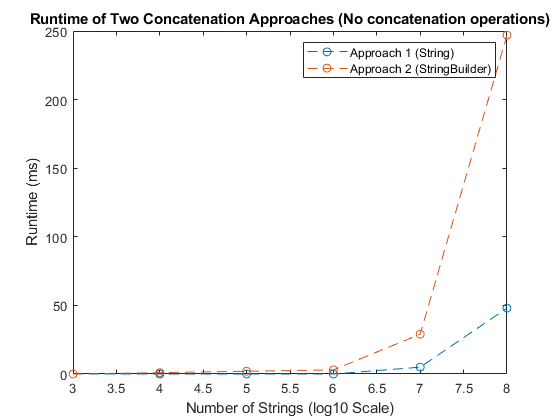
\includegraphics[width=\textwidth]{3b.png}

3c) The number of concatenation operations need to be two to guarantee that Approach 2 (StringBuilder) has faster runtime than Approach 1 (String) for each test with different number of Strings. As the number of Strings increases, it amplifies the difference between two approaches, where 1000000 Strings is critical point that starts to show significant difference. The result is consistent with the result in 2b). Approach 1 experiences performance issue as the number of concatenation operations increasem, and the increase in number of Strings amplifies the performance issue further.

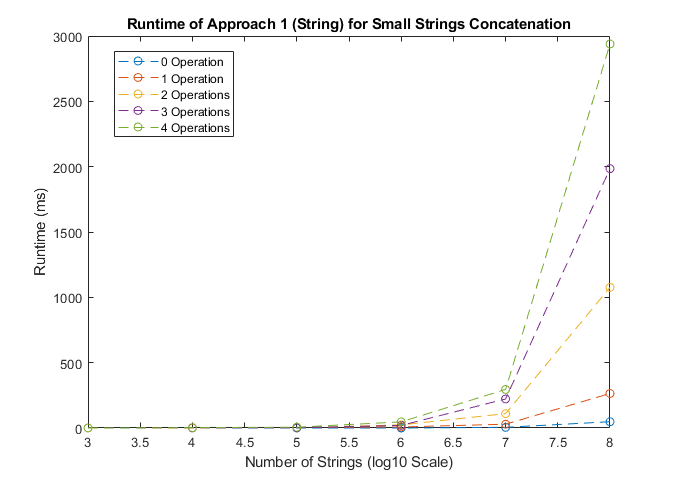
\includegraphics[width=\textwidth]{3cA1.png}

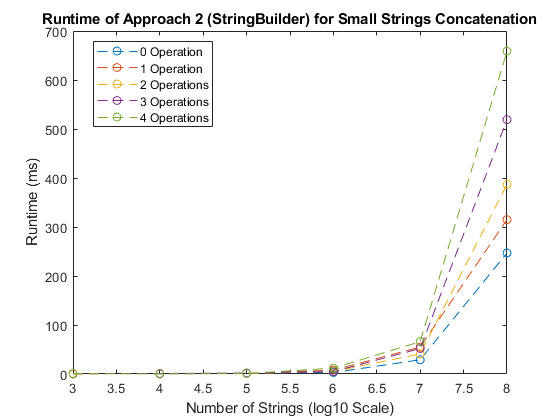
\includegraphics[width=\textwidth]{3cA2.png}

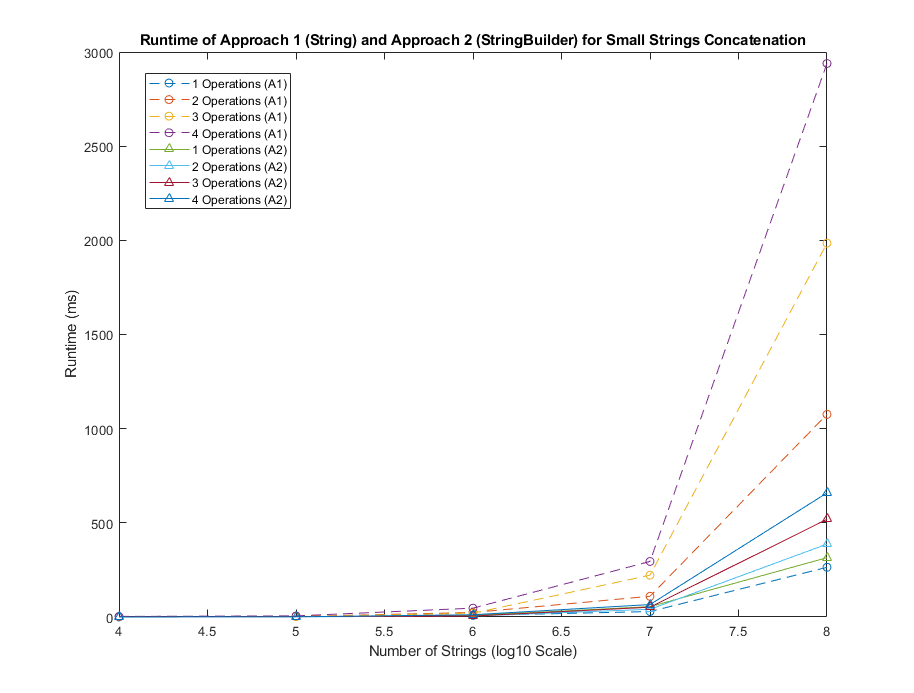
\includegraphics[width=\textwidth]{3cT.png}



\end{document}